% Created by tikzDevice version 0.12.3 on 2020-09-01 22:15:38
% !TEX encoding = UTF-8 Unicode
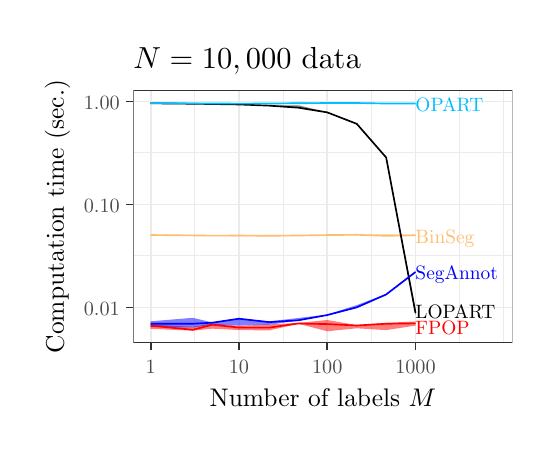
\begin{tikzpicture}[x=1pt,y=1pt]
\definecolor{fillColor}{RGB}{255,255,255}
\path[use as bounding box,fill=fillColor,fill opacity=0.00] (0,0) rectangle (180.67,144.54);
\begin{scope}
\path[clip] (  0.00,  0.00) rectangle (180.67,144.54);
\definecolor{drawColor}{RGB}{255,255,255}
\definecolor{fillColor}{RGB}{255,255,255}

\path[draw=drawColor,line width= 0.6pt,line join=round,line cap=round,fill=fillColor] ( -0.00,  0.00) rectangle (180.67,144.54);
\end{scope}
\begin{scope}
\path[clip] ( 38.23, 30.69) rectangle (175.17,121.88);
\definecolor{fillColor}{RGB}{255,255,255}

\path[fill=fillColor] ( 38.23, 30.69) rectangle (175.17,121.88);
\definecolor{drawColor}{gray}{0.92}

\path[draw=drawColor,line width= 0.3pt,line join=round] ( 38.23, 62.09) --
	(175.17, 62.09);

\path[draw=drawColor,line width= 0.3pt,line join=round] ( 38.23, 99.30) --
	(175.17, 99.30);

\path[draw=drawColor,line width= 0.3pt,line join=round] ( 60.40, 30.69) --
	( 60.40,121.88);

\path[draw=drawColor,line width= 0.3pt,line join=round] ( 92.30, 30.69) --
	( 92.30,121.88);

\path[draw=drawColor,line width= 0.3pt,line join=round] (124.20, 30.69) --
	(124.20,121.88);

\path[draw=drawColor,line width= 0.3pt,line join=round] (156.09, 30.69) --
	(156.09,121.88);

\path[draw=drawColor,line width= 0.3pt,line join=round] (172.04, 30.69) --
	(172.04,121.88);

\path[draw=drawColor,line width= 0.6pt,line join=round] ( 38.23, 43.48) --
	(175.17, 43.48);

\path[draw=drawColor,line width= 0.6pt,line join=round] ( 38.23, 80.69) --
	(175.17, 80.69);

\path[draw=drawColor,line width= 0.6pt,line join=round] ( 38.23,117.91) --
	(175.17,117.91);

\path[draw=drawColor,line width= 0.6pt,line join=round] ( 44.45, 30.69) --
	( 44.45,121.88);

\path[draw=drawColor,line width= 0.6pt,line join=round] ( 76.35, 30.69) --
	( 76.35,121.88);

\path[draw=drawColor,line width= 0.6pt,line join=round] (108.25, 30.69) --
	(108.25,121.88);

\path[draw=drawColor,line width= 0.6pt,line join=round] (140.14, 30.69) --
	(140.14,121.88);
\definecolor{fillColor}{RGB}{253,191,111}

\path[fill=fillColor,fill opacity=0.50] ( 44.45, 69.85) --
	( 59.67, 69.52) --
	( 66.75, 69.51) --
	( 76.35, 69.52) --
	( 87.27, 69.64) --
	( 97.79, 69.57) --
	(108.25, 69.60) --
	(118.92, 69.69) --
	(129.54, 69.99) --
	(140.14, 69.67) --
	(140.14, 69.32) --
	(129.54, 69.20) --
	(118.92, 69.57) --
	(108.25, 69.57) --
	( 97.79, 69.23) --
	( 87.27, 69.20) --
	( 76.35, 69.14) --
	( 66.75, 69.23) --
	( 59.67, 69.37) --
	( 44.45, 69.44) --
	cycle;

\path[] ( 44.45, 69.85) --
	( 59.67, 69.52) --
	( 66.75, 69.51) --
	( 76.35, 69.52) --
	( 87.27, 69.64) --
	( 97.79, 69.57) --
	(108.25, 69.60) --
	(118.92, 69.69) --
	(129.54, 69.99) --
	(140.14, 69.67);

\path[] (140.14, 69.32) --
	(129.54, 69.20) --
	(118.92, 69.57) --
	(108.25, 69.57) --
	( 97.79, 69.23) --
	( 87.27, 69.20) --
	( 76.35, 69.14) --
	( 66.75, 69.23) --
	( 59.67, 69.37) --
	( 44.45, 69.44);
\definecolor{fillColor}{RGB}{255,0,0}

\path[fill=fillColor,fill opacity=0.50] ( 44.45, 37.23) --
	( 59.67, 36.45) --
	( 66.75, 37.65) --
	( 76.35, 36.77) --
	( 87.27, 37.30) --
	( 97.79, 37.85) --
	(108.25, 38.91) --
	(118.92, 37.06) --
	(129.54, 37.90) --
	(140.14, 38.38) --
	(140.14, 36.88) --
	(129.54, 35.25) --
	(118.92, 35.91) --
	(108.25, 34.83) --
	( 97.79, 37.56) --
	( 87.27, 35.14) --
	( 76.35, 35.27) --
	( 66.75, 35.77) --
	( 59.67, 35.06) --
	( 44.45, 35.71) --
	cycle;

\path[] ( 44.45, 37.23) --
	( 59.67, 36.45) --
	( 66.75, 37.65) --
	( 76.35, 36.77) --
	( 87.27, 37.30) --
	( 97.79, 37.85) --
	(108.25, 38.91) --
	(118.92, 37.06) --
	(129.54, 37.90) --
	(140.14, 38.38);

\path[] (140.14, 36.88) --
	(129.54, 35.25) --
	(118.92, 35.91) --
	(108.25, 34.83) --
	( 97.79, 37.56) --
	( 87.27, 35.14) --
	( 76.35, 35.27) --
	( 66.75, 35.77) --
	( 59.67, 35.06) --
	( 44.45, 35.71);
\definecolor{fillColor}{RGB}{0,0,0}

\path[fill=fillColor,fill opacity=0.50] ( 44.45,117.53) --
	( 59.67,117.05) --
	( 66.75,117.04) --
	( 76.35,116.84) --
	( 87.27,116.37) --
	( 97.79,116.50) --
	(108.25,113.98) --
	(118.92,109.80) --
	(129.54, 97.82) --
	(140.14, 43.13) --
	(140.14, 40.74) --
	(129.54, 97.47) --
	(118.92,109.70) --
	(108.25,113.88) --
	( 97.79,115.59) --
	( 87.27,116.35) --
	( 76.35,116.78) --
	( 66.75,116.93) --
	( 59.67,117.00) --
	( 44.45,117.11) --
	cycle;

\path[] ( 44.45,117.53) --
	( 59.67,117.05) --
	( 66.75,117.04) --
	( 76.35,116.84) --
	( 87.27,116.37) --
	( 97.79,116.50) --
	(108.25,113.98) --
	(118.92,109.80) --
	(129.54, 97.82) --
	(140.14, 43.13);

\path[] (140.14, 40.74) --
	(129.54, 97.47) --
	(118.92,109.70) --
	(108.25,113.88) --
	( 97.79,115.59) --
	( 87.27,116.35) --
	( 76.35,116.78) --
	( 66.75,116.93) --
	( 59.67,117.00) --
	( 44.45,117.11);
\definecolor{fillColor}{RGB}{0,191,255}

\path[fill=fillColor,fill opacity=0.50] ( 44.45,117.43) --
	( 59.67,117.24) --
	( 66.75,117.18) --
	( 76.35,117.13) --
	( 87.27,117.12) --
	( 97.79,117.74) --
	(108.25,117.33) --
	(118.92,117.58) --
	(129.54,117.30) --
	(140.14,117.25) --
	(140.14,117.10) --
	(129.54,117.11) --
	(118.92,117.26) --
	(108.25,117.28) --
	( 97.79,117.10) --
	( 87.27,117.11) --
	( 76.35,117.10) --
	( 66.75,117.10) --
	( 59.67,117.14) --
	( 44.45,117.24) --
	cycle;

\path[] ( 44.45,117.43) --
	( 59.67,117.24) --
	( 66.75,117.18) --
	( 76.35,117.13) --
	( 87.27,117.12) --
	( 97.79,117.74) --
	(108.25,117.33) --
	(118.92,117.58) --
	(129.54,117.30) --
	(140.14,117.25);

\path[] (140.14,117.10) --
	(129.54,117.11) --
	(118.92,117.26) --
	(108.25,117.28) --
	( 97.79,117.10) --
	( 87.27,117.11) --
	( 76.35,117.10) --
	( 66.75,117.10) --
	( 59.67,117.14) --
	( 44.45,117.24);
\definecolor{fillColor}{RGB}{0,0,255}

\path[fill=fillColor,fill opacity=0.50] ( 44.45, 38.43) --
	( 59.67, 39.70) --
	( 66.75, 38.01) --
	( 76.35, 39.40) --
	( 87.27, 38.41) --
	( 97.79, 39.62) --
	(108.25, 40.88) --
	(118.92, 44.28) --
	(129.54, 48.28) --
	(140.14, 56.49) --
	(140.14, 56.03) --
	(129.54, 48.03) --
	(118.92, 43.25) --
	(108.25, 40.67) --
	( 97.79, 38.70) --
	( 87.27, 37.20) --
	( 76.35, 36.89) --
	( 66.75, 37.25) --
	( 59.67, 36.20) --
	( 44.45, 36.36) --
	cycle;

\path[] ( 44.45, 38.43) --
	( 59.67, 39.70) --
	( 66.75, 38.01) --
	( 76.35, 39.40) --
	( 87.27, 38.41) --
	( 97.79, 39.62) --
	(108.25, 40.88) --
	(118.92, 44.28) --
	(129.54, 48.28) --
	(140.14, 56.49);

\path[] (140.14, 56.03) --
	(129.54, 48.03) --
	(118.92, 43.25) --
	(108.25, 40.67) --
	( 97.79, 38.70) --
	( 87.27, 37.20) --
	( 76.35, 36.89) --
	( 66.75, 37.25) --
	( 59.67, 36.20) --
	( 44.45, 36.36);
\definecolor{drawColor}{RGB}{253,191,111}

\path[draw=drawColor,line width= 0.6pt,line join=round] ( 44.45, 69.61) --
	( 59.67, 69.47) --
	( 66.75, 69.38) --
	( 76.35, 69.43) --
	( 87.27, 69.34) --
	( 97.79, 69.44) --
	(108.25, 69.60) --
	(118.92, 69.69) --
	(129.54, 69.32) --
	(140.14, 69.53);
\definecolor{drawColor}{RGB}{255,0,0}

\path[draw=drawColor,line width= 0.6pt,line join=round] ( 44.45, 36.86) --
	( 59.67, 35.38) --
	( 66.75, 37.20) --
	( 76.35, 36.17) --
	( 87.27, 36.16) --
	( 97.79, 37.64) --
	(108.25, 37.43) --
	(118.92, 36.92) --
	(129.54, 37.55) --
	(140.14, 37.70);
\definecolor{drawColor}{RGB}{0,0,0}

\path[draw=drawColor,line width= 0.6pt,line join=round] ( 44.45,117.21) --
	( 59.67,117.05) --
	( 66.75,116.94) --
	( 76.35,116.79) --
	( 87.27,116.36) --
	( 97.79,115.63) --
	(108.25,113.93) --
	(118.92,109.79) --
	(129.54, 97.62) --
	(140.14, 41.41);
\definecolor{drawColor}{RGB}{0,191,255}

\path[draw=drawColor,line width= 0.6pt,line join=round] ( 44.45,117.30) --
	( 59.67,117.18) --
	( 66.75,117.13) --
	( 76.35,117.10) --
	( 87.27,117.12) --
	( 97.79,117.23) --
	(108.25,117.31) --
	(118.92,117.31) --
	(129.54,117.13) --
	(140.14,117.11);
\definecolor{drawColor}{RGB}{0,0,255}

\path[draw=drawColor,line width= 0.6pt,line join=round] ( 44.45, 37.56) --
	( 59.67, 37.55) --
	( 66.75, 37.94) --
	( 76.35, 39.38) --
	( 87.27, 38.14) --
	( 97.79, 38.80) --
	(108.25, 40.69) --
	(118.92, 43.48) --
	(129.54, 48.13) --
	(140.14, 56.26);
\end{scope}
\begin{scope}
\path[clip] ( 38.23, 30.69) rectangle (175.17,121.88);
\definecolor{drawColor}{RGB}{255,0,0}

\node[text=drawColor,anchor=base west,inner sep=0pt, outer sep=0pt, scale=  0.70] at (140.14, 33.77) {FPOP};
\definecolor{drawColor}{RGB}{0,0,0}

\node[text=drawColor,anchor=base west,inner sep=0pt, outer sep=0pt, scale=  0.70] at (140.14, 39.56) {LOPART};
\definecolor{drawColor}{RGB}{0,0,255}

\node[text=drawColor,anchor=base west,inner sep=0pt, outer sep=0pt, scale=  0.70] at (140.14, 53.37) {SegAnnot};
\definecolor{drawColor}{RGB}{253,191,111}

\node[text=drawColor,anchor=base west,inner sep=0pt, outer sep=0pt, scale=  0.70] at (140.14, 66.63) {BinSeg};
\definecolor{drawColor}{RGB}{0,191,255}

\node[text=drawColor,anchor=base west,inner sep=0pt, outer sep=0pt, scale=  0.70] at (140.14,114.21) {OPART};
\definecolor{drawColor}{gray}{0.20}

\path[draw=drawColor,line width= 0.6pt,line join=round,line cap=round] ( 38.23, 30.69) rectangle (175.17,121.88);
\end{scope}
\begin{scope}
\path[clip] (  0.00,  0.00) rectangle (180.67,144.54);
\definecolor{drawColor}{gray}{0.30}

\node[text=drawColor,anchor=base east,inner sep=0pt, outer sep=0pt, scale=  0.73] at ( 33.28, 40.45) {0.01};

\node[text=drawColor,anchor=base east,inner sep=0pt, outer sep=0pt, scale=  0.73] at ( 33.28, 77.66) {0.10};

\node[text=drawColor,anchor=base east,inner sep=0pt, outer sep=0pt, scale=  0.73] at ( 33.28,114.88) {1.00};
\end{scope}
\begin{scope}
\path[clip] (  0.00,  0.00) rectangle (180.67,144.54);
\definecolor{drawColor}{gray}{0.20}

\path[draw=drawColor,line width= 0.6pt,line join=round] ( 35.48, 43.48) --
	( 38.23, 43.48);

\path[draw=drawColor,line width= 0.6pt,line join=round] ( 35.48, 80.69) --
	( 38.23, 80.69);

\path[draw=drawColor,line width= 0.6pt,line join=round] ( 35.48,117.91) --
	( 38.23,117.91);
\end{scope}
\begin{scope}
\path[clip] (  0.00,  0.00) rectangle (180.67,144.54);
\definecolor{drawColor}{gray}{0.20}

\path[draw=drawColor,line width= 0.6pt,line join=round] ( 44.45, 27.94) --
	( 44.45, 30.69);

\path[draw=drawColor,line width= 0.6pt,line join=round] ( 76.35, 27.94) --
	( 76.35, 30.69);

\path[draw=drawColor,line width= 0.6pt,line join=round] (108.25, 27.94) --
	(108.25, 30.69);

\path[draw=drawColor,line width= 0.6pt,line join=round] (140.14, 27.94) --
	(140.14, 30.69);
\end{scope}
\begin{scope}
\path[clip] (  0.00,  0.00) rectangle (180.67,144.54);
\definecolor{drawColor}{gray}{0.30}

\node[text=drawColor,anchor=base,inner sep=0pt, outer sep=0pt, scale=  0.73] at ( 44.45, 19.68) {1};

\node[text=drawColor,anchor=base,inner sep=0pt, outer sep=0pt, scale=  0.73] at ( 76.35, 19.68) {10};

\node[text=drawColor,anchor=base,inner sep=0pt, outer sep=0pt, scale=  0.73] at (108.25, 19.68) {100};

\node[text=drawColor,anchor=base,inner sep=0pt, outer sep=0pt, scale=  0.73] at (140.14, 19.68) {1000};
\end{scope}
\begin{scope}
\path[clip] (  0.00,  0.00) rectangle (180.67,144.54);
\definecolor{drawColor}{RGB}{0,0,0}

\node[text=drawColor,anchor=base,inner sep=0pt, outer sep=0pt, scale=  0.92] at (106.70,  7.64) {Number of labels $M$};
\end{scope}
\begin{scope}
\path[clip] (  0.00,  0.00) rectangle (180.67,144.54);
\definecolor{drawColor}{RGB}{0,0,0}

\node[text=drawColor,rotate= 90.00,anchor=base,inner sep=0pt, outer sep=0pt, scale=  0.92] at ( 13.08, 76.28) {Computation time (sec.)};
\end{scope}
\begin{scope}
\path[clip] (  0.00,  0.00) rectangle (180.67,144.54);
\definecolor{drawColor}{RGB}{0,0,0}

\node[text=drawColor,anchor=base west,inner sep=0pt, outer sep=0pt, scale=  1.10] at ( 38.23,129.95) {$N=10,000$ data};
\end{scope}
\end{tikzpicture}
